\chapter{An algorithm for testing pattern-avoidance of a general pattern}
\label{chap:general}
In this chapter and Chapter \ref{chap:walking} we show algorithms for testing whether a pattern $P$ is contained in a square binary matrix $M$.

We begin with a very basic algorithm, which we then improve a lot to get a fast algorithm for testing avoidance of a general pattern.

\section{Sketch of a brute force algorithm}
Let $L=(l_1,l_2,\cdots,l_{w+h-1})$ be a permutation of lines (rows and columns) of the pattern $P$ and $k\in[w+h-1]$. \emph{Partial mapping of level $k$} of lines of $P$ is a function $f$ from $L':=\{l_1,l_2,\cdots,l_k\}\subseteq L$ to lines of the big matrix $M$ satisfying three conditions: 
%The basic algorithm we use goes as follows. It takes a line $l$ (row or column) of the pattern and for each line $L$ of the big matrix it decides whether the pattern can be mapped there. It can, if three conditions are all met at once:
\begin{itemize}
%\item Both $l$ and $L$ are rows or they are both columns.
%\item If $l'$ is a line of $P$ parallel to $l$ that has been mapped previously to line $L'$, we want $l<l'\Leftrightarrow L<L'$. This means we want the mapped lines to be in the same order as they were in the pattern.
%\item If $l'$ is a line of the pattern orthogonal to $l$ that has been mapped previously to line $L'$ and there is a one-entry at the intersection of $l$ and $l'$, there has to be one-entry at the intersection of $L$ and $L'$.
\item Both $l'\in L'$ and $f(l')$ are rows or they are both columns.
\item If $l'\in L'$ and $l''\in L'$ are both rows or columns and $l'<l''$, then $f(l')<f(l'')$. This means partial mapping keeps the order of the lines.
\item If $l'\in L'$ is a row of $P$ and $l''\in L'$ is a column of $P$ and there is a one-entry at the intersection of $l'$ and $l''$, then there is a one-entry at the intersection of $f(l')$ and $f(l'')$.
\end{itemize}
The basic algorithm we use goes as follows. First it maps $l_1$ to all possible lines of $M$, creating partial mappings of $\{l_1\}\subseteq L$. For $k=2,\cdots,w+h-1$ it takes each partial mapping from the previous iteration and extends it by adding line $l_k$ to the partial mapping in all possible ways. If we manage to map all the lines of $P$, then $M$ does not avoid it and if at some point there are no partial mappings to extend it means $M$ avoids $P$.

The algorithm can be improved in two ways. Firstly, we can try to recognize unextendable partial mappings earlier than at the moment a line can no longer be mapped, for example by counting whether there is enough one-entries in between already mapped lines (more in Section \ref{sect:approaches}). Secondly, which is going to be fundamental for us, we can try not to remember more copies of different mappings that can be extended in the same way.

\section{Equivalent mappings}
There is no need to remember two different partial mappings of the same level if they can be both extended exactly the same way, because our function is only supposed to check whether a pattern can be mapped to a big matrix not to find all such mappings.
\begin{defn}
We call a line $l$ of a pattern $P$ \emph{important} for chosen permutation of lines of $P$, if one of the conditions is met:
\begin{itemize}
\item An adjacent line of the pattern has not been mapped yet.
\item There is a one-entry on the line $l$ at the intersection with line $l'$ that has not been mapped yet.
\end{itemize}.
Otherwise the line is \emph{unimportant} for the permutation.
\end{defn}
Whether a line is important or not only depends on the permutation, so if we have a line unimportant in a partial mapping of level $k$, it is unimportant in every partial mapping of level $k$.

At the beginning, when no line is mapped, all lines are important. After some lines get mapped, a line can become unimportant in the partial mapping as all lines that bound it are in the mapping as well. If a line is unimportant in a partial mapping of some level, it will stay unimportant in all extensions of the mapping we can find.
\begin{defn}
We say two partial mappings of the same level are \emph{equivalent} if all important lines in the mapping of that level are mapped to the same lines of the big matrix in both mappings.
\end{defn}
\begin{figure}[h!]
\centering
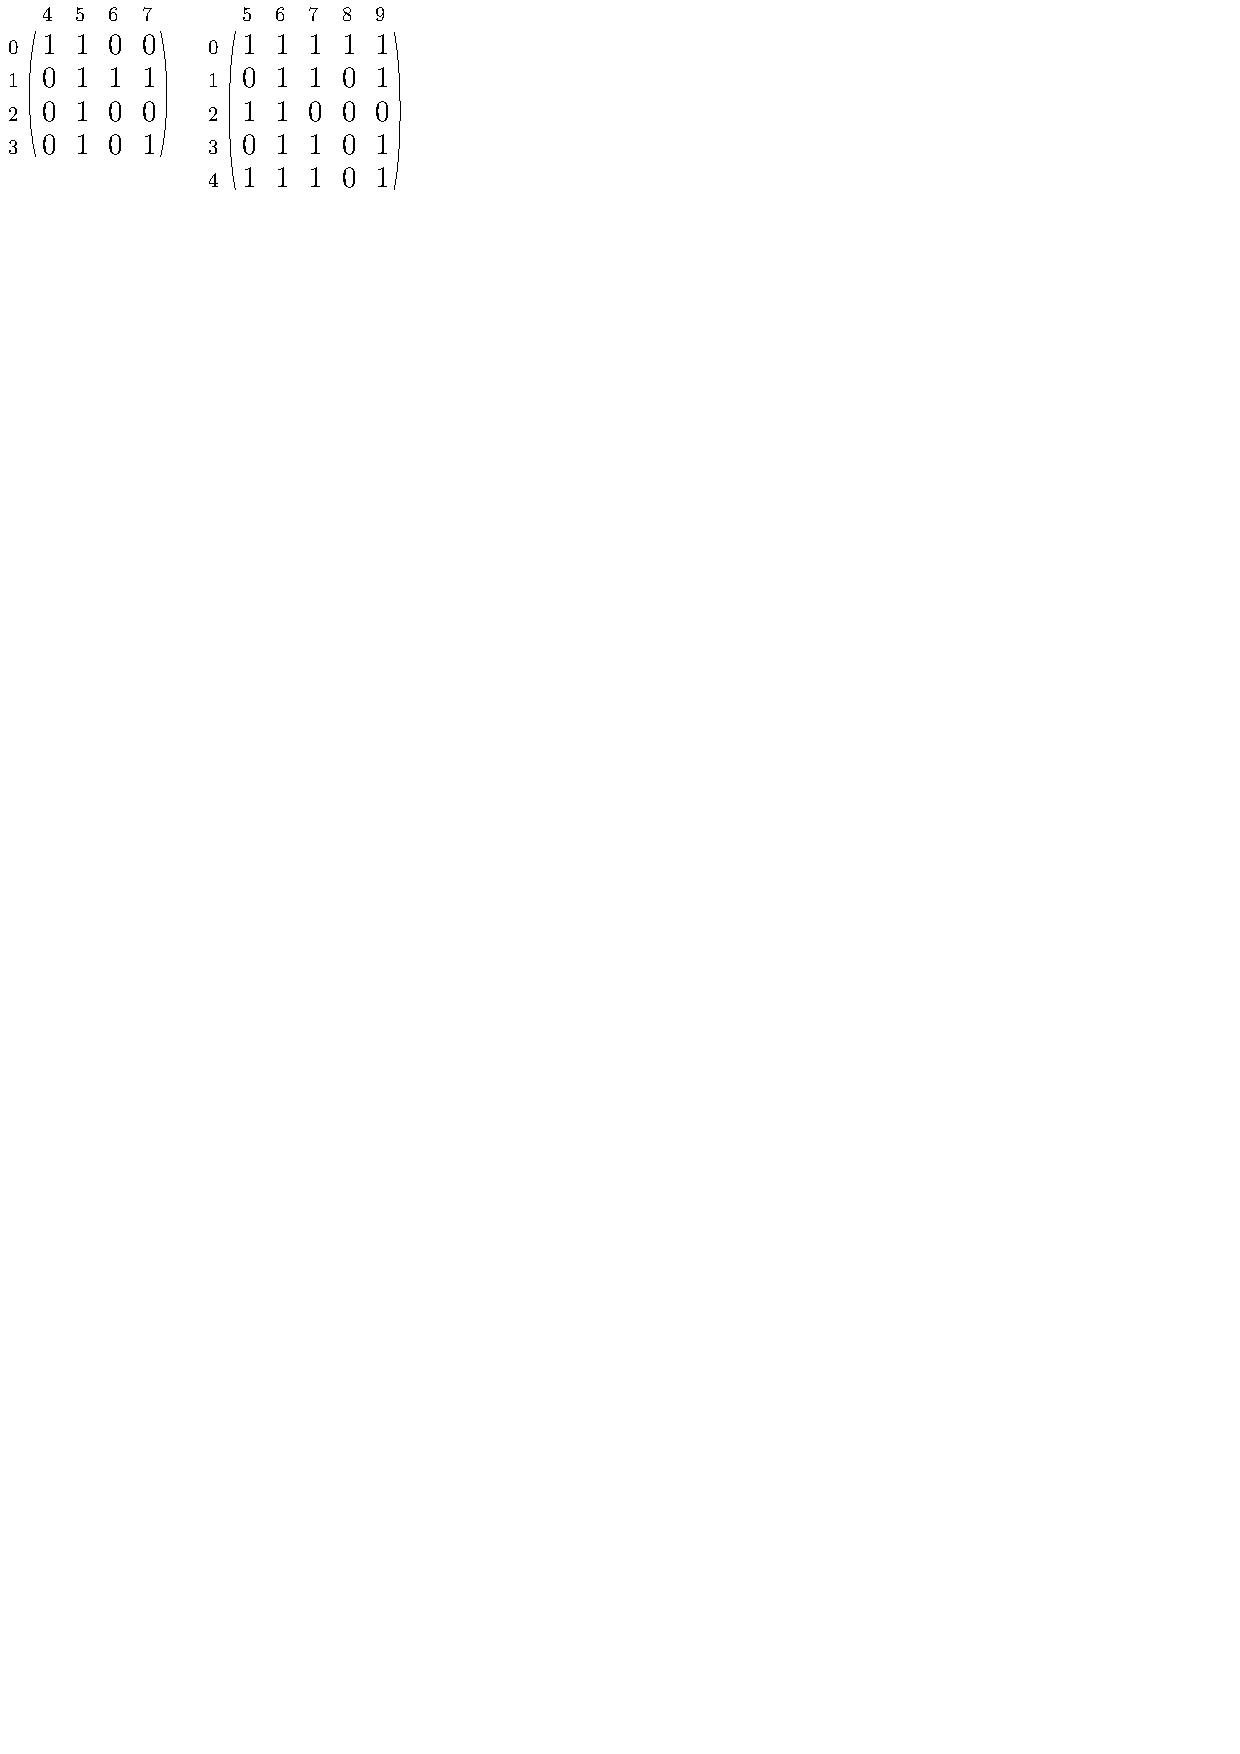
\includegraphics[width=100mm]{../img/equivalent.pdf}
\caption{An example showing unimportant line and equivalent mappings.}
\label{equivalent}
\end{figure}
%\centerline{\mbox{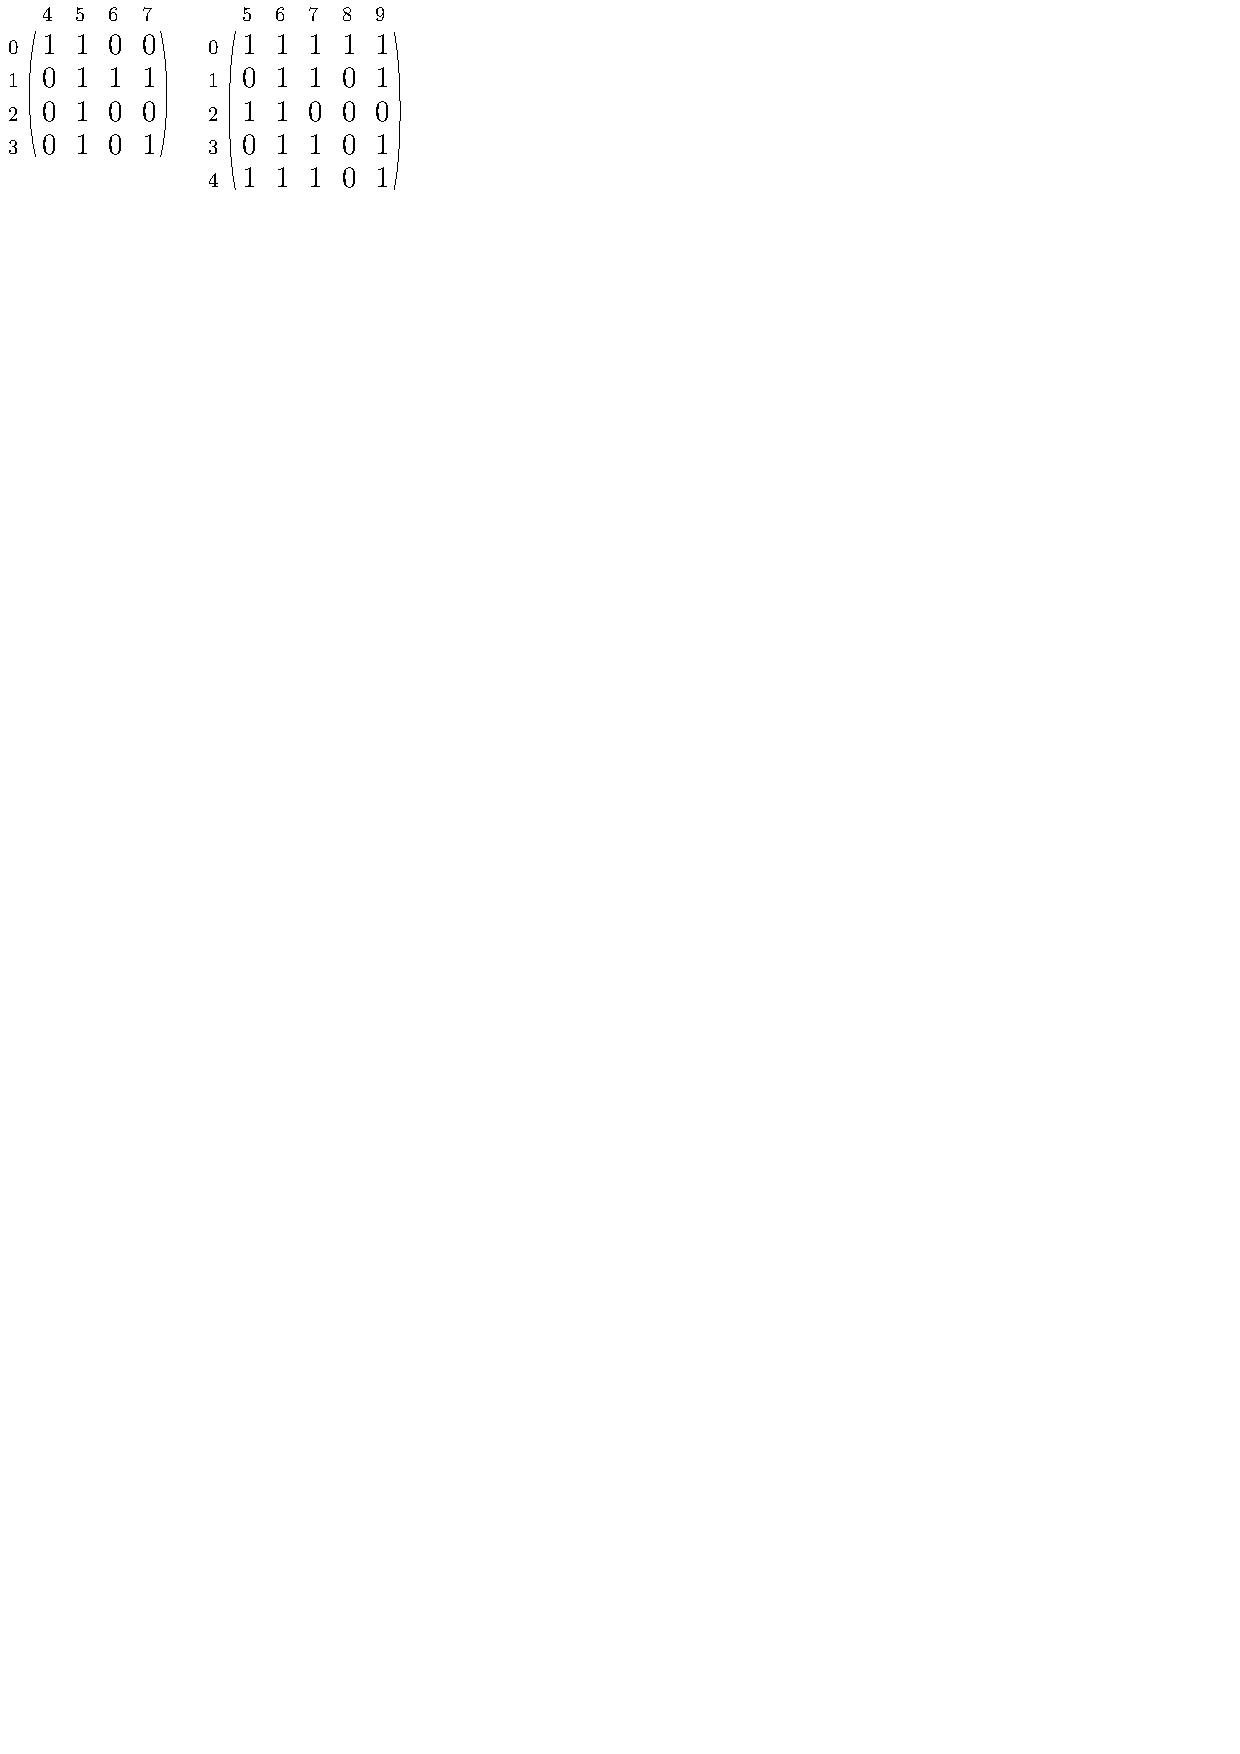
\includegraphics[width=100mm]{../img/equivalent.pdf}}}
For $P$ and $M$, binary matrices in Figure \ref{equivalent}, in partial mapping of level $4$ $f=\{(1,1),(2,2),(3,4),(5,6)\}$, line $2$ is unimportant because both lines $1$ and $3$ are mapped and so is line $5$ - the only line to intersect line $2$ in a one-entry. Line $3$ is important, because there is line $7$ intersecting it in one-entry, which is not mapped.

In the same situation as above, consider a different partial mapping $f'=\{(1,1),(2,3),(3,4),(5,6)\}$, which is a mapping of the same level as $f$ and only differs from $f$ in mapping line $2$. The line $2$ is unimportant and by the definition of equivalent partial mappings, $f$ and $f'$ are equivalent. The idea behind this notion is simple. It is not important where we map line $2$, because it does not restrict where we can map any other line that has not been mapped yet. This means that if a partial mapping $f$ can be somehow extended, the equivalent partial mapping $f'$ can be extended in the same way; therefore, it is sufficient to only extend one of them in order to find one full mapping. Note that it would be also sufficient to only extend one of the partial mappings if we were looking for all full mappings, but, in that case, we would need to keep the information about where the unimportant lines were mapped to.